\section{Izoxorik jarayon}


\begin{enumerate}

\item Izoxorik jarayon deb qanday jarayonga aytiladi?
\begin{enumerate}[label=\Alph*)]
\item doimiy bosim ostida...
\item doimiy hajmda...
\item doimiy haroratda...
\item issiqlik almashmasdan...
\end{enumerate}

\item Ballondagi gazning temperaturasi 288 K, bosimi 18 atm. Temperatura qanday bo‘lganda gazning bosimi 15,5 atm ga teng bo‘ladi (K)? Balloning hajmi o‘zgarmas deb hisoblang.
\begin{enumerate}[label=\Alph*)]
\item 326
\item 562
\item 124
\item 248
\end{enumerate}

\item $-13^\circ C$ temperaturada avtomobil kamerasida havoning bosimi 160 kPa edi. Avtomobil uzoq vaqt harakatlanishi natijasida havo $37^\circ C$ gacha qiziydi. Shunda bosim qancha bo‘ladi (kPa)?
\begin{enumerate}[label=\Alph*)]
\item 190
\item 220
\item 420
\item 18
\end{enumerate}

\item Yopiq idishda $27^\circ C$ haroratli 75 kPa bosimda ideal gaz bor. Shu gazning $-13^\circ C$ haroratdagi bosimini toping (kPa).
\begin{enumerate}[label=\Alph*)]
\item 37,5
\item 40
\item 50
\item 65
\end{enumerate}

\item Ideal gazning temperaturasi izoxorik ravishda $6^\circ C$ ga ko‘tarilganda, gaz bosimi dastlabki qiymatining 1/50 qismiga oshdi. Gazning dastlabki temperaturasini toping ($^\circ C$).
\begin{enumerate}[label=\Alph*)]
\item 27
\item 50
\item 127
\item 300
\end{enumerate}

\item Temperaturasi $0^\circ C$ bo‘lgan gazning bosimini $n$ marta orttirish uchun uni qanday temperaturagacha o‘zgarmas hajmda qizdirish kerak ($^\circ C$)?
\begin{enumerate}[label=\Alph*)]
\item $273(n-1)$
\item $273n$
\item $373(n-1)$
\item $373n$
\end{enumerate}

\item Agar ballondagi ideal gaz temperaturasi 300 K ga ko‘tarilganda, bosim 3 marta ortgan bo‘lsa, uning dastlabki temperaturasi necha kelvin bo‘lgan?
\begin{enumerate}[label=\Alph*)]
\item 300
\item 250
\item 100
\item 150
\end{enumerate}

\item Ballondagi gazni 150 K ga isitilganda, uning bosimi 2 marta oshgan. Gazning boshlang‘ich temperaturasi nimaga teng bo‘lgan?
\begin{enumerate}[label=\Alph*)]
\item 300
\item 400
\item 200
\item 150
\end{enumerate}

\item Ballonga o‘rnatilgan manometr 2,8 atm qiymatni ko‘rsatib turgan edi, temperatura $85^\circ C$ kamayganda uning ko‘rsatishi 1 atm kamaydi. Ikkala holdagi temperatura qiymatini aniqlang ($^\circ C$). Protsess—izoxorik.
\begin{enumerate}[label=\Alph*)]
\item 80; -35
\item 50; -26
\item 50; 35
\item -120; -35
\end{enumerate}

\item Berk idishdagi $27^\circ C$ temperaturali gazning bosimi 2 marta oshishi uchun temperaturani necha gradus ko‘tarish kerak?
\begin{enumerate}[label=\Alph*)]
\item 27
\item 54
\item 300
\item 600
\end{enumerate}

\item O‘zgarmas hajmda gaz harorati 1 K ga isitilganda gazning bosimi 0,5 \% ga oshgan. Gazning dastlabki harorati ($^\circ C$) qanday bo‘lgan?
\begin{enumerate}[label=\Alph*)]
\item 72
\item -73
\item -23
\item 47
\end{enumerate}

\item Ballondagi argon gazi ishlatilishi davomida gazning massasi 20 \%, bosimi esa 2 marta kamaygan bo‘lsa, uning harorati dastlabki haroratga nisbatan necha marta kamaygan?
\begin{enumerate}[label=\Alph*)]
\item 1,25
\item 1,6
\item 2,5
\item 5
\end{enumerate}

\item P-T grafikda keltirilgan izoxoralarning qaysi birida gaz hajmi eng katta?

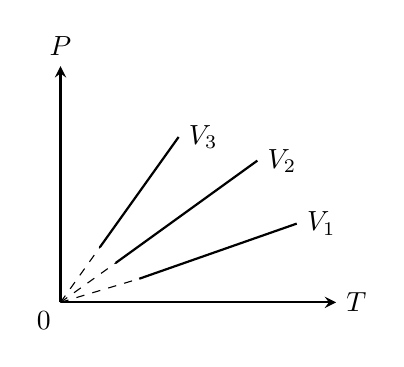
\begin{tikzpicture}[>=stealth, scale=1]
    % Koordinata o'qlari
    \draw[->, thick] (0,0) -- (3.5,0) node[right] {$T$};
    \draw[->, thick] (0,0) -- (0,3) node[above] {$P$};
    \node[below left] at (0,0) {0};

    % Izoxoralarni chizish (P = (nR/V)*T chiziqli funksiya)
    % Izoxora V3 (eng katta qiyalik - eng kichik hajm)
    \draw[dashed] (0,0) -- (0.5, 0.7);
    \draw[thick] (0.5, 0.7) -- (1.5, 2.1) node[right] {$V_3$};
    
    % Izoxora V2 (o'rtacha qiyalik)
    \draw[dashed] (0,0) -- (0.7, 0.5);
    \draw[thick] (0.7, 0.5) -- (2.5, 1.8) node[right] {$V_2$};
    
    % Izoxora V1 (eng kichik qiyalik - eng katta hajm)
    \draw[dashed] (0,0) -- (1, 0.3);
    \draw[thick] (1, 0.3) -- (3, 1) node[right] {$V_1$};

\end{tikzpicture}

\begin{enumerate}[label=\Alph*)]
\item $V_3$
\item $V_2$
\item $V_1$
\item Hammasining hajmlari teng
\end{enumerate}

\item Rasmda bir xil massali ideal gaz uchun uchta izoxora keltirilgan. Ulardan qaysi biri eng kichik hajmga mos keladi?

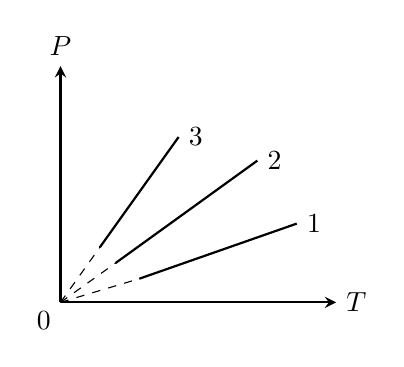
\begin{tikzpicture}[>=stealth, scale=1]
    % Koordinata o'qlari
    \draw[->, thick] (0,0) -- (3.5,0) node[right] {$T$};
    \draw[->, thick] (0,0) -- (0,3) node[above] {$P$};
    \node[below left] at (0,0) {0};

    % Izoxoralarni chizish (P = (nR/V)*T chiziqli funksiya)
    % Izoxora V3 (eng katta qiyalik - eng kichik hajm)
    \draw[dashed] (0,0) -- (0.5, 0.7);
    \draw[thick] (0.5, 0.7) -- (1.5, 2.1) node[right] {$3$};
    
    % Izoxora V2 (o'rtacha qiyalik)
    \draw[dashed] (0,0) -- (0.7, 0.5);
    \draw[thick] (0.7, 0.5) -- (2.5, 1.8) node[right] {$2$};
    
    % Izoxora V1 (eng kichik qiyalik - eng katta hajm)
    \draw[dashed] (0,0) -- (1, 0.3);
    \draw[thick] (1, 0.3) -- (3, 1) node[right] {$1$};

\end{tikzpicture}

\begin{enumerate}[label=\Alph*)]
\item 2
\item 1
\item uchala holda ham hajm bir xil
\item 3
\end{enumerate}

\item Qaysi tenglama izoxorik jarayonni ifodalaydi?
\begin{enumerate}[label=\Alph*)]
\item $p = nkT$
\item $p/T = const.$
\item $pV = const.$
\item $V/T = const.$
\end{enumerate}

\item Ideal gazning bosimi izoxorik ravishda 2 marta ortdi, so`ngra izotermik ravishda bosimi ikki marta ortguncha siqildi. Bu ikki jaroyonda gaz hajmi necha marta o`zgargan?


\begin{enumerate}[label=\Alph*)]
\item 2 marta ortgan
\item 2 marta kamaygan
\item 4 marta ortgan
\item 4 marta kamaygan
\end{enumerate}

\item Ideal gaz bosimining termik koeffitsiyenti qanday?
\begin{enumerate}[label=\Alph*)]
\item $V / (V_0 T)$
\item $\Delta V / V_0$
\item $\Delta p / (p_0 \Delta T)$
\item $p / (p_0 T)$
\end{enumerate}

\item Gazning zichligi $\rho \sim T^{-1}$ bo‘lgan jarayonda temperatura ortishi bilan gazning bosimi qanday o‘zgaradi?
\begin{enumerate}[label=\Alph*)]
\item o‘zgarmaydi
\item avval kamayadi, keyin ortadi
\item ortadi
\item kamayadi
\end{enumerate}

\item Gaz qamalgan ballondagi manometr $17^\circ C$ temperaturali xonada 240 kPa bosimni ko‘rsatadi. Ko‘chada esa manometr ko‘rsatishi 40 kPa kamaygan. Agar atmosfera bosimi 100 kPa bo‘lsa, tashqaridagi havo temperaturasini toping ($^\circ C$).
\begin{enumerate}[label=\Alph*)]
\item -52
\item -29
\item 256
\item -33
\end{enumerate}

\item Gaz bosimi 293 K da $1,07 \cdot 10^5$ Pa ga teng. Agar gazni o‘zgarmas hajmda 423 K gacha qizdirilgandagi va o‘zgarmas bosimda 250 K gacha sovitilgandagi gaz bosimlari yig‘indisini toping (Pa).
\begin{enumerate}[label=\Alph*)]
\item $2,61 \cdot 10^5$
\item $1,65 \cdot 10^4$
\item $2,45 \cdot 10^2$
\item $2,46 \cdot 10^5$
\end{enumerate}

\item Germetik bo‘lmagan idishdagi gazning absolyut temperaturasi 25 \% oshirildi. Gaz konsentratsiyasi necha foizga kamayadi?
\begin{enumerate}[label=\Alph*)]
\item 20
\item 15
\item 30
\item 25
\end{enumerate}

\item Silindrik idishdagi porshen ostida ideal gaz bor. Gazning absolyut harorati 1,5 marta oshirilganda porshen avvalgi holatida qolishi uchun uning ustiga 8 kg massali yuk qo‘yish kerak bo‘ldi. Agar porshenning yuzi 10 $sm^2$ bo‘lsa, gazning dastlabki bosimini (kPa) aniqlang. $g=10 m/s^2$.
\begin{enumerate}[label=\Alph*)]
\item 100
\item 160
\item 132
\item 80
\end{enumerate}

\item Silindrik idishdagi porshen ostida ideal gaz bor. Gazning absolyut harorati 1,8 marta oshirilganda porshen avvalgi vaziyatida qolishi uchun uning ustiga 12 kg massali yuk qo‘yish kerak bo‘ladi. Agar porshenning yuzi 10 $sm^2$ bo‘lsa, gazning dastlabki bosimini (kPa) aniqlang. $g=10 m/s^2$.
\begin{enumerate}[label=\Alph*)]
\item 150
\item 109
\item 132
\item 160
\end{enumerate}

\end{enumerate}



\begin{table}[h!]
\centering
\begin{tabular}{|c|c|c|c|c|c|c|c|c|c|}
\hline
№ & J. & № & J. & № & J. & № & J. & № & J. \\ \hline
1 & B & 6 & A & 11 & B & 16 & B & 21 & A \\ \hline
2 & D & 7 & D & 12 & B & 17 & C & 22 & B \\ \hline
3 & A & 8 & D & 13 & C & 18 & A & 23 & A \\ \hline
4 & D & 9 & D & 14 & D & 19 & D & & \\ \hline
5 & A & 10 & C & 15 & B & 20 & A & & \\ \hline
\end{tabular}
\end{table}